\documentclass{report}
\usepackage[english]{babel}
\usepackage[utf8]{inputenc}
\usepackage[T1]{fontenc}
\usepackage{listings}
\usepackage{titlesec}
\usepackage{color}
\usepackage{graphicx}
\usepackage{geometry}
\geometry{hmargin=2.5cm,vmargin=3.5cm}

\titleformat{\chapter}[display]
            {\normalfont\bfseries}{}{0pt}{\Huge}

\lstset{ escapeinside={(*}{*)} }

\title{\textbf{Rapport IHM PROG6}\\Pingouin}

\author{Castel Antonin, Reboul Paul, Soret Louka, Sorin Gaëtan, Vandendorpe Thomas}
\begin{document}

\maketitle{}
\tableofcontents
\chapter{Introduction}
bla bla bla
\chapter{Menu}.
\section{Truc}
blabla

\section{Truc}
blabla

%pour les espaces:
%\hspace{0.5cm}
%\vspace{0.7cm}

\chapter{Scene de jeu}
La scène de jeu se décompose en 4 parties principales: la plateau, les scores, la panneau d'information, les paramètres/options.

\begin{figure}
\begin{center}
   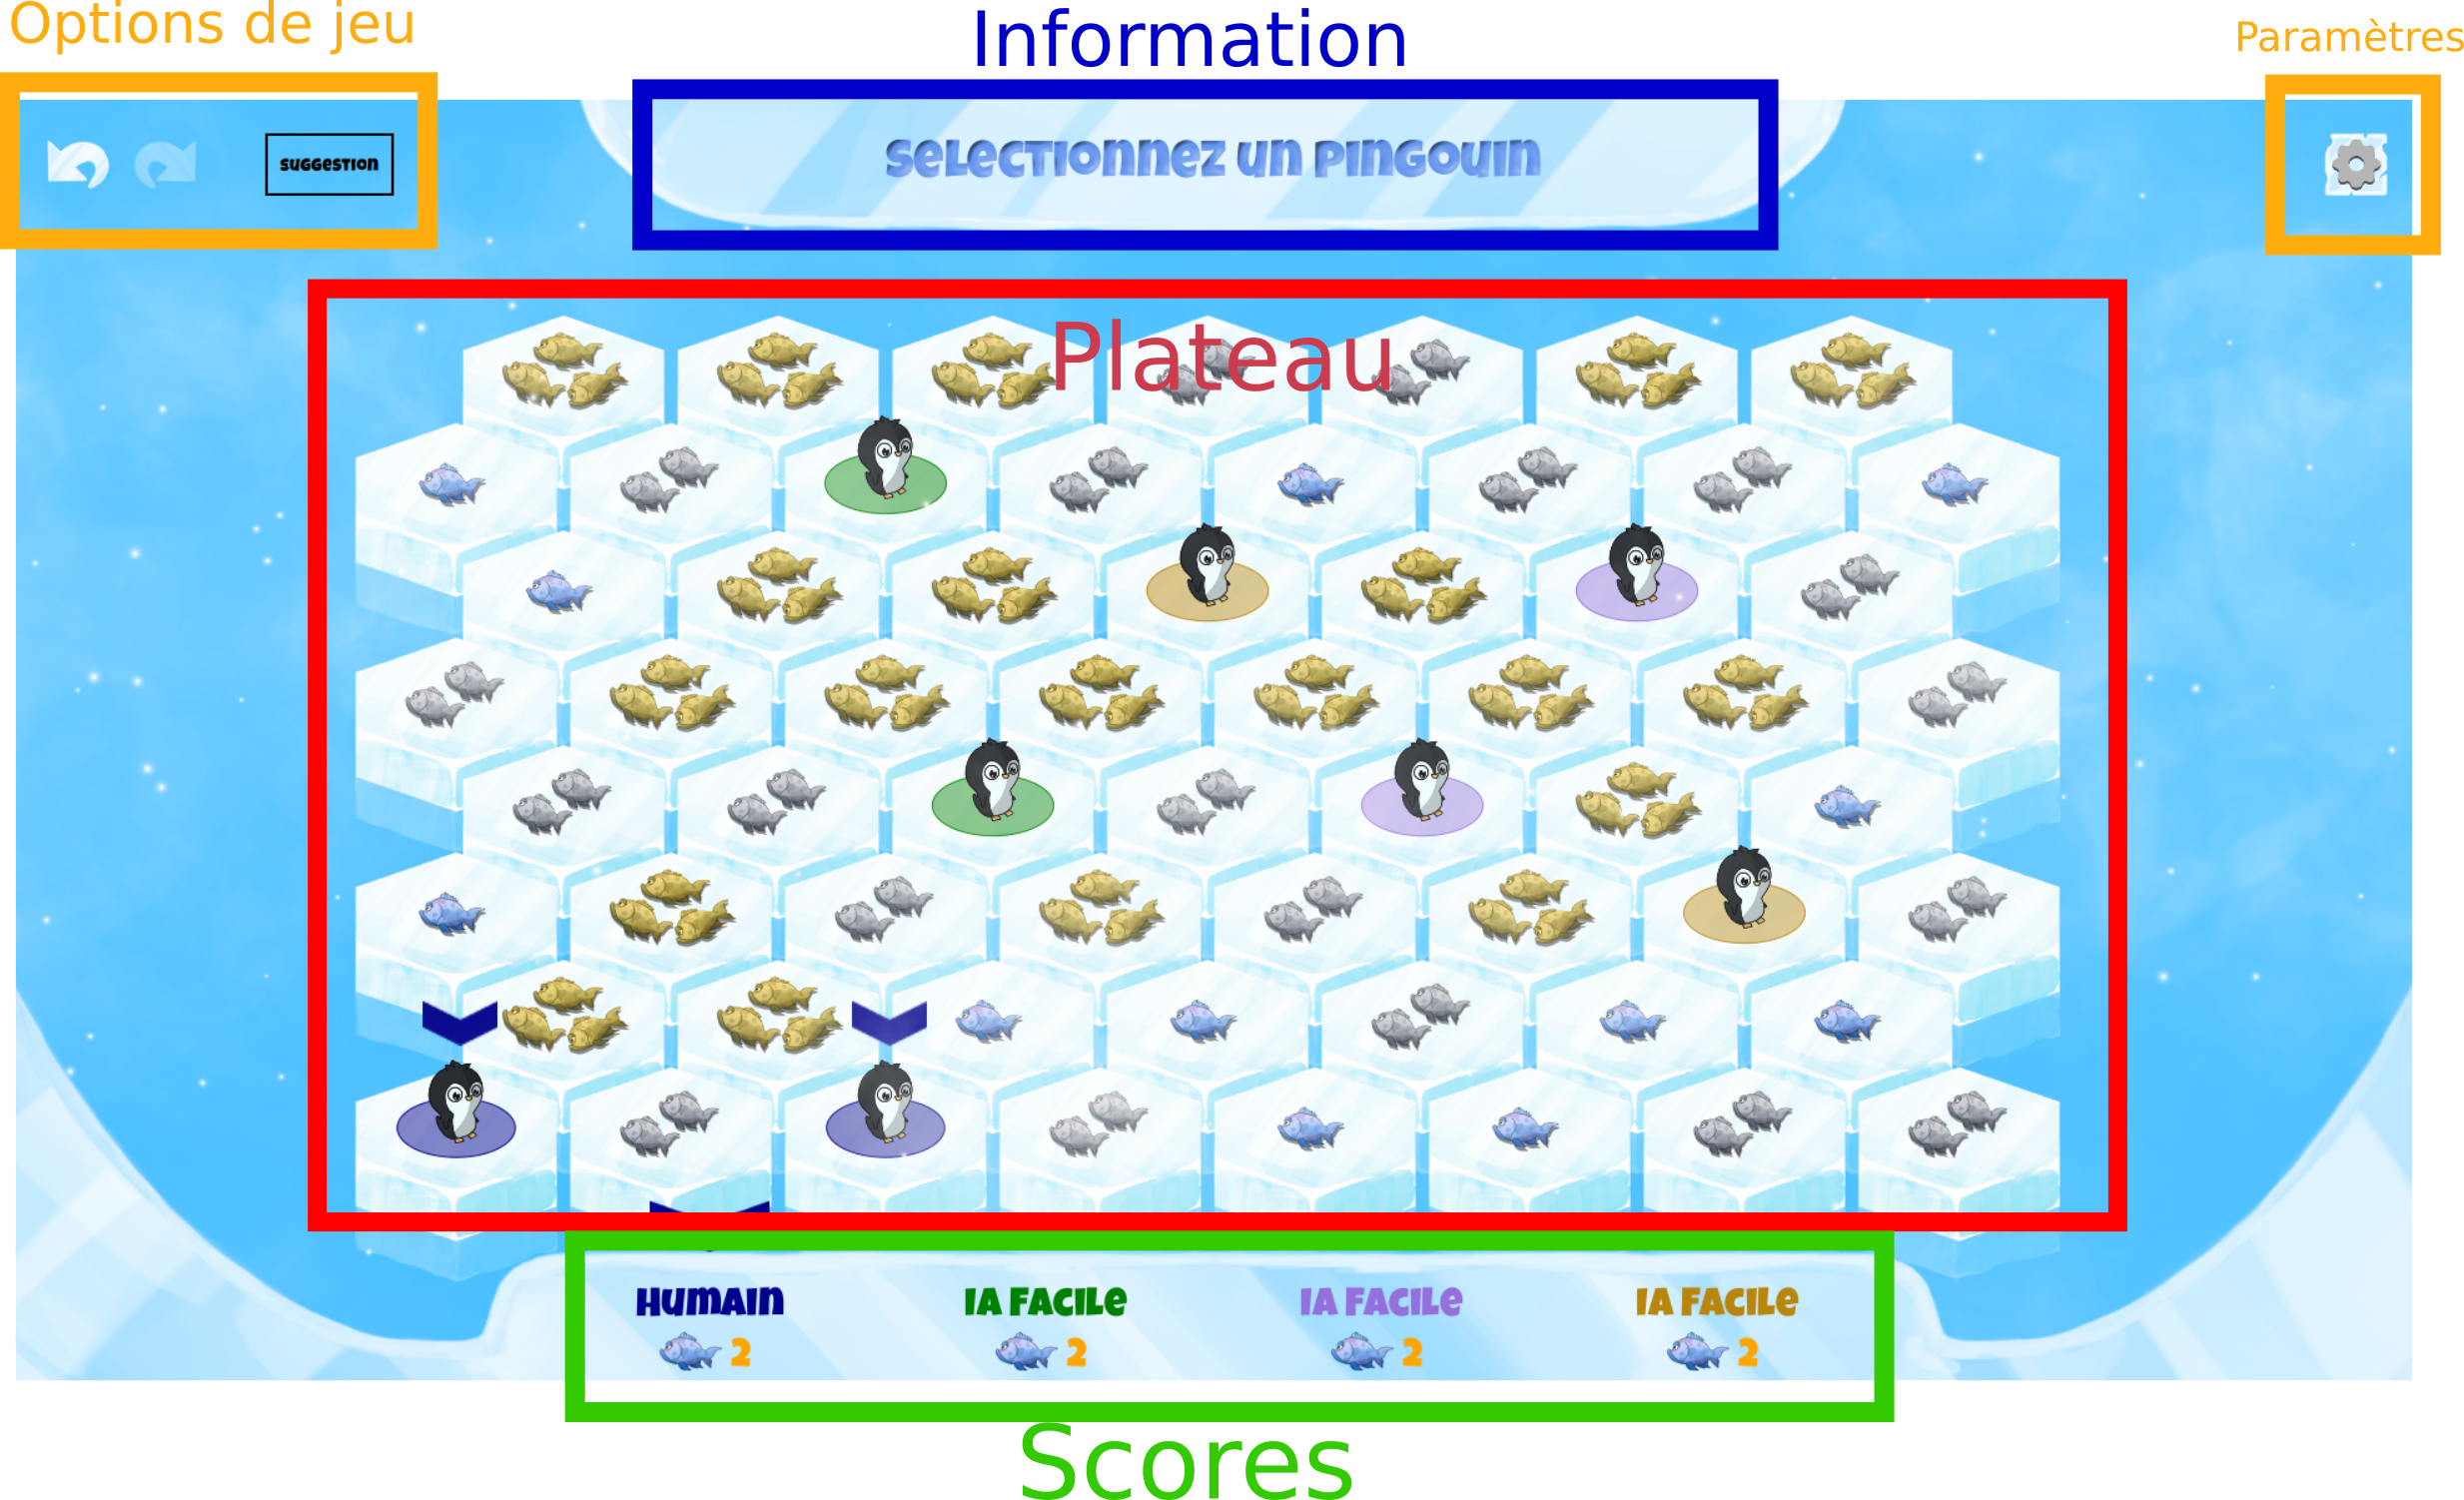
\includegraphics[width=20cm]{image/plateauIHM.png}    
\end{center}
\caption{Scene de jeu}
\end{figure}

\section{Plateau}
Le plateau est évidemment l'élément pincipal, c'est pourquoi c'est l'élément le plus grand et qu'il est centré. Cependant beaucoup d'intéractions sont possible avec ce plateau. Suite aux tests IHM,
nous avons constaté que les joueurs, lors de la première utilisation du jeu, comprennent mieux les éléments intéractifs si ces derniers sont dynamiques (clignotement, mouvement, ...). Voici comment nous avons mis en évidence les actions possibles au différentes phases du jeu.

\begin{itemize}
\item Poser un pingouin: mise en évidence des cases à 1 poissons lors de la phase de pose des pingouins. La couleur de la case est de la couleur du joueur courant et clignote pour signaler un objet avec lequel on peut interragir.
  \begin{center}
    
    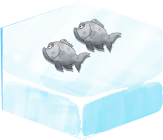
\includegraphics[width=1.5cm]{image/bloc_simple.png}    
    \hspace{1cm}
    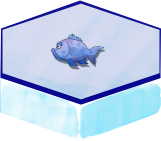
\includegraphics[width=1.5cm]{image/bloc_mev.png}
    \\
    bloc non cliquable \hspace{0.5cm} bloc cliquable
  \end{center}

\item Selectionner un pingouin: les pingouins sont tous identifiés par des ronds de la couleur de son joueur en dessous de lui. Nous avons ensuite rajouté une flèche sur les pingouins déplaçable du joueur courant. Ces flèches bouge indiquant qu'on peut intéragir avec le pingouin.
  \begin{center}
    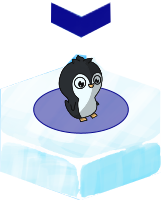
\includegraphics[width=1.5cm]{image/bloc_pingouin.png}    
  \end{center}

\item Sélectionner destinnation: le pingouin séléctionné est mis en valeur, et les cases prennent la même forme que pour la pose des pingouins.
\begin{center}
   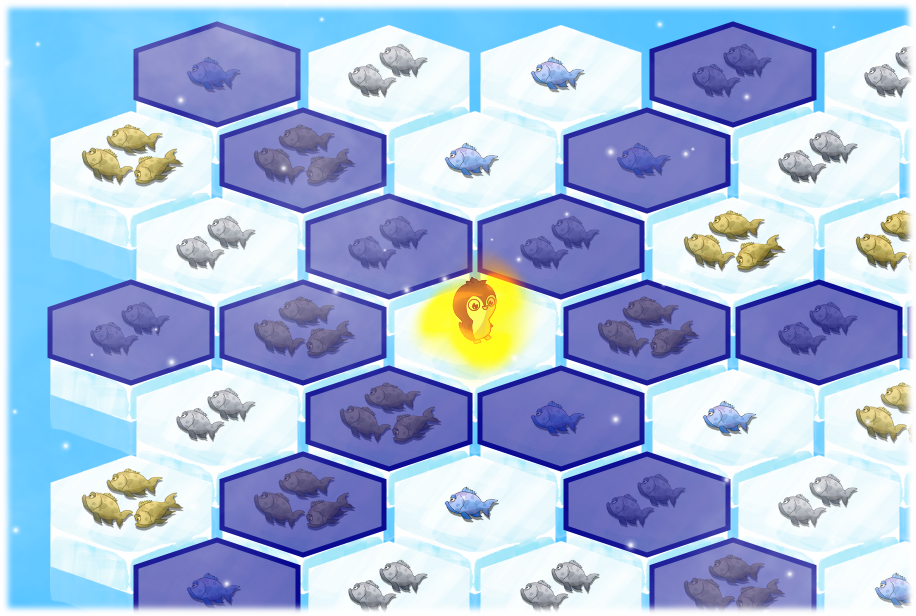
\includegraphics[width=4cm]{image/case_select_dest.png}    
\end{center}

\item Déplacement des pingouins: lorsqu'on joue contre l'IA, il est important de montrer au joueur l'action qu'est en train de faire l'IA. Nous avons optez pour une animation lors du déplacement, les contraintes étaient d'avoir une animation visible, mais aussi rapide car si le jeu devient trop lent, il devient ennuyant pour l'utilisateur. Ainsi lorsque le pingouin de l'IA s'apprète à bouger, il s'enflamme, puis se téléporte à sa case destinnation en laissant une trainée de flammes derrière lui.
  \begin{center}
    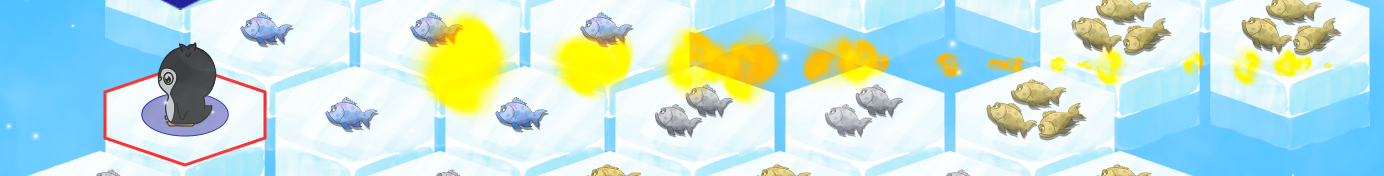
\includegraphics[width=8cm]{image/pingouin_deplacement.png}    
  \end{center}
  Nous avons géré le delai de l'animation en fonction des retours utilisateurs, lors des tests IHM, nous avons testé plusieurs delais et pris celui qui convenait satisfaisait le plus le plus de joueurs.
\end{itemize}

\section{Panneau des scores}
Le joueurs doit connaître plusieurs information concernant l'état courant du jeu. Le panneau des scores en bas de la scène regroupe le nom des joueurs, leurs scores (nombre de poissons mangés), ainsi que le nombre de pingouin qu'il reste à poser (lors de la phase de pose des pingouins). On se sert également de ce panneau pour indiquer le joueur courant à l'aide d'une flêche, bien que nous nous somme rendu compte que les utilisateurs regarde plutôt les informations du plateau (flèche au dessus des pingouins) pour savoir qui doit jouer.
  \begin{center}
    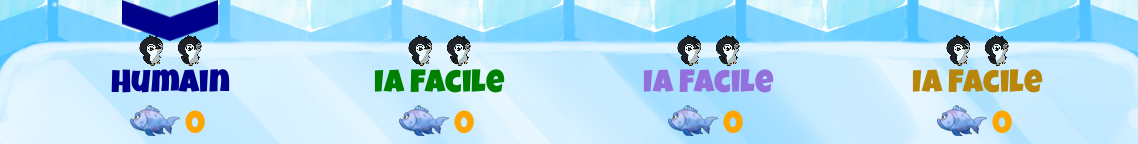
\includegraphics[width=8cm]{image/tableau_scores.png}    
  \end{center}

\section{Panneau d'information}
Nous avons souhaité qu'un joueur puisse constamment savoir qu'elle action il doit faire (même s'il ne connait pas les règles du jeu). C'est pourquoi, en plus d'avoir des éléments dynamique sur le plateau l'insitant à intéragir, il existe aussi un panneau informant de ce que doit faire le joueur: ``Poser un pingouin'', ``Selectionner un pingouin'', ``Selectionner une destinnation'', ``Attendre son tour''. Au fil des tests utilisateurs, nous avons dû augmenter la taille du panneau afin de le mettre plus en évidence. En effet nous avons pu constater que tous les utilisateurs n'ont pas le réflex de lire alors que ce panneau peut être important lors des premières parties d'un joueur.

\section{Paramètres et options}
Nous avons choisi de placer les boutons non essentiels au jeu au même endroit qu'on peut les trouver dans d'autre logiciel, afin de ne pas trop changer les habitudes des utilisateurs. Nous avons donc le undo/redo en haut à gauche et les paramètres en haut à droite. Voici quelques remarques interessantes concernant ces options:

\begin{itemize}
\item Boutons grisés: Certains des boutons peuvent parfois ne pas être activable, ils sont donc grisé dans ce cas.


\end{itemize}
\end{document}
